%%%%%%%%%%%%%%%%%%%%%%%%%%%%%%%%%%%%%%%%%%%%%%%%%%%%%%%%%%%%%%%%%%%%%%%%%%%%%%%%
% Preámbulo                                                                    %
%%%%%%%%%%%%%%%%%%%%%%%%%%%%%%%%%%%%%%%%%%%%%%%%%%%%%%%%%%%%%%%%%%%%%%%%%%%%%%%%
\documentclass[10pt,a4paper,titlepage,oneside]{report}

%%% RELACIÓN DE VARIABLES A PERSONALIZAR %%%
%\def\lingua{gal}
\def\lingua{esp} % descomenta esta liña se redactarás a memoria en español
%\def\lingua{eng} % descomenta esta liña se redactarás a memoria en inglés
\def\nomeA{Óscar Olveira Miniño}
\def\nomeB{Alejandro Javier Herrero Arango}                     % substitúe aquí o teu nome
%\def\nomedirectorB{Outro Nome Completo}             % duplica esta liña máis veces se o precisas, cambiando
                                                     % a letra final (A, B, C, D...): úsanse na portada.tex
\def\titulo{Práctica 3: MANETs en INET} % substitúe aquí o título do teu TFG
%\def\titulacion{gced}                               % descomenta esta liña e comenta a seguinte se es estudante do GCED
\def\titulacion{gei}
%\def\mencion{COMPUTACIÓN}                           % descomenta a mención que che corresponda se es estudante do GEI
%\def\mencion{ENXEÑARÍA DO SOFTWARE}
%\def\mencion{ENXEÑARÍA DE COMPUTADORES}
%\def\mencion{SISTEMAS DE INFORMACIÓN}
\def\mencion{TECNOLOXÍAS DA INFORMACIÓN}

%\def\renomearcadros{si} % descomenta esta liña se redactas a memoria en español e prefires que
                         % os "cuadros" e o "índice de cuadros" se renomeen
                         % a "tablas" e "índice de tablas" respectivamente

\usepackage{estilo_tfg}
\usepackage{tcolorbox}
\usepackage{float}
% Lista de paquetes potencialmente interesantes (uso baixo demanda)

% \usepackage{alltt}       % proporciona o entorno alltt, semellante a verbatim pero que respecta comandos
% \usepackage{enumitem}    % permite personalizar os entornos de lista
% \usepackage{eurofont}    % proporciona o comando \euro
% \usepackage{float}       % permite máis opcións para controlar obxectos flotantes (táboas, figuras)
% \usepackage{hhline}      % permite personalizar as liñas horizontais en arrays e táboas
\usepackage{longtable}   % permite construir táboas que ocupan máis dunha páxina
\usepackage{geometry}
\geometry{a4paper, left=2.75cm, right=2.25cm, top=2.5cm, bottom=2.5cm}
\usepackage{hyperref}
% \usepackage{lscape}      % permite colocar partes do documento en orientación apaisada
% \usepackage{moreverb}    % permite personalizar o entorno verbatim
% \usepackage{multirow}    % permite crear celdas que ocupan varias filas da mesma táboa
% \usepackage{pdfpages}    % permite insertar ficheiros en PDF no documento
% \usepackage{rotating}    % permite diferentes tipos de rotacións para figuras e táboas
% \usepackage{subcaption}  % permite a inclusión de varias subfiguras nunha figura
% \usepackage{tabu}        % permite táboas flexibles
% \usepackage{tabularx}    % permite táboas con columnas de anchura determinada

%%%%%%%%%%%%%%%%%%%%%%%%%%%%%%%%%%%%%%%%%%%%%%%%%%%%%%%%%%%%%%%%%%%%%%%%%%%%%%%%
% Corpo                                                                        %
%%%%%%%%%%%%%%%%%%%%%%%%%%%%%%%%%%%%%%%%%%%%%%%%%%%%%%%%%%%%%%%%%%%%%%%%%%%%%%%%

\begin{document}

 %%%%%%%%%%%%%%%%%%%%%%%%%%%%%%%%%%%%%%%%
 % Preliminares do documento            %
 %%%%%%%%%%%%%%%%%%%%%%%%%%%%%%%%%%%%%%%%

 \begin{titlepage}
  
  \hspace*{128pt}
  \textcolor{udcpink}{{\fontencoding{T1}\fontfamily{phv}\selectfont Facultade de Informática}}\\[-32pt]

  \begin{center}
    
\includegraphics[scale=0.3]{imaxes/udc}\\[25pt]

    {\large TRABALLO FIN DE GRAO \\
            \nometitulacion \\
            \nomemencion } \\[10pt]

    \carimbo \\[25pt]

    \begin{huge}
      \begin{spacing}{1.3}
        \bfseries \titulo
      \end{spacing}
    \end{huge}
  \end{center}
  
  \vfill
  
  \begin{flushright}
    {\large
    \begin{tabular}{ll}
      {\bf Estudante 1:}& \nomeA\\
      {\bf Estudante 2:}& \nomeB
%                      & \nomedirectorB \\ % duplica esta liña máis veces se o precisas, cambiando
                                           % a letra final (A, B, C, D...); define eses nomes no memoria_tfg.tex
    \end{tabular}}
  \end{flushright}
  \rightline{A Coruña, \datasimple.}
\end{titlepage}

 %\dedicatoria{Dedicatoria} % escribe neste comando o teu texto de dedicatoria
 %\paxinaenbranco
 %\begin{agradecementos}
 %\blindtext                % substitúe este comando polo teu texto de agradecementos
 %\end{agradecementos}
 %%%%%%%%%%%%%%%%%%%%%%%%%%%%%%%%%%%%%%%%%%%%%%%%%%%%%%%%%%%%%%%%%%%%%%%%%%%%%%%%%

\pagestyle{empty}
\begin{abstract}
  \blindtext % substitúe este comando polo resumo do teu TFG
             % na lingua principal do documento (tipicamente: galego)

  \vspace*{25pt}
  \begin{segundoresumo}
    \blindtext % substitúe este comando polo resumo do teu TFG
               % na lingua secundaria do documento (tipicamente: inglés)
  \end{segundoresumo}
\vspace*{25pt}
\begin{multicols}{2}
\begin{description}
\item [\palabraschaveprincipal:] \mbox{} \\[-20pt]
  \blindlist{itemize}[7] % substitúe este comando por un itemize
                         % que relacione as palabras chave
                         % que mellor identifiquen o teu TFG
                         % no idioma principal da memoria (tipicamente: galego)
\end{description}
\begin{description}
\item [\palabraschavesecundaria:] \mbox{} \\[-20pt]
  \blindlist{itemize}[7] % substitúe este comando por un itemize
                         % que relacione as palabras chave
                         % que mellor identifiquen o teu TFG
                         % no idioma secundario da memoria (tipicamente: inglés)
\end{description}
\end{multicols}

\end{abstract}
\pagestyle{fancy}

%%%%%%%%%%%%%%%%%%%%%%%%%%%%%%%%%%%%%%%%%%%%%%%%%%%%%%%%%%%%%%%%%%%%%%%%%%%%%%%%


 \pagenumbering{roman}
 \setcounter{page}{1}
 \bstctlcite{IEEEexample:BSTcontrol}

 \setcounter{tocdepth}{1}
 \tableofcontents
 \listoffigures
 %\listoftables
 \clearpage
 
 \pagenumbering{arabic}
 \setcounter{page}{1}

 %%%%%%%%%%%%%%%%%%%%%%%%%%%%%%%%%%%%%%%%
 % Capítulos                            %
 %%%%%%%%%%%%%%%%%%%%%%%%%%%%%%%%%%%%%%%%

 \chapter{AODV}
\label{chap:aodv}

\section{Ejercicio 1.1}

\subsection{¿Qué nodos reenvían el primer paquete RREQ enviado por static1? ¿Y el segundo RREQ? ¿Por qué?}

El primer paquete RREQ enviado por static1 es recibido y reenviado únicamente por los nodos mobile[10] y mobile [12], a pesar de enviarse con intención de alcanzar todos los nodos de la red (Figura \ref{fig:primer_rreq_reception}). Esto ocurre porque el primer envío contiene un TTL igual a 2 (aparece en la documentación de Inet), por lo que solamente van a responder los dispositivos a los que le llegue un TTL > 1 para asi poder hacer el reenvío.

El segundo RREQ es reenviado por 10, 12, 3, 1, 7, 2. Al hacer el segundo reenvío, el TTL del paquete pasa a ser 4 (según la documentación de INET, en los siguientes paquetes, el TTL se suma 2 con respeto al anterior ya que el objetivo es poder llegar lo más lejos posible). Como ahora el TLL es 4, pasa por 10 y 12 otra vez (el TTL pasa a ser 3), 12 no alcanza ningún objetivo pero 10 logra mandar ese paquete a 1 y 3 (el TTL pasa a ser 2) y como 3 llega alcanzar a 7 y 2, se los envía también. Llegados a este punto, el TTL es 1 por lo que ya que se acabaría todos los posibles reenvíos del segundo RREQ.

\begin{figure}[H]
    \centering
    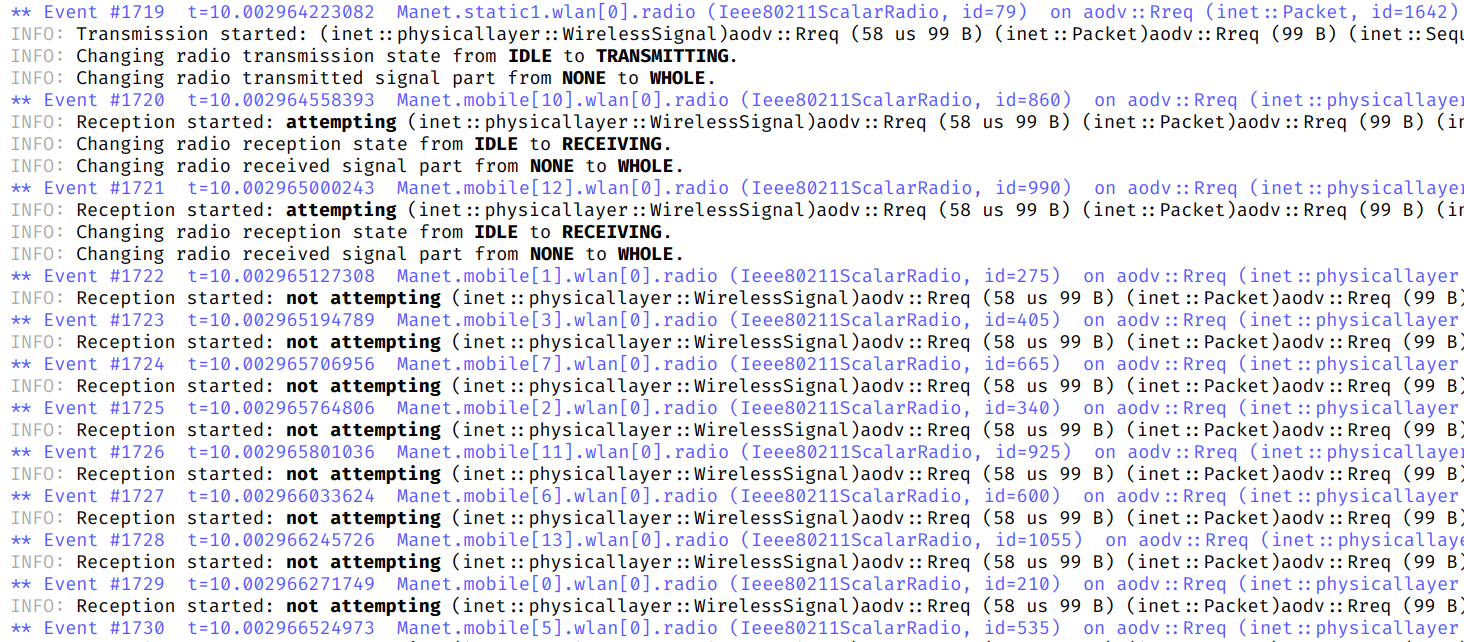
\includegraphics[width=135mm, scale=0.75]{imaxes/ejercicio1_1.png}
    \caption{Logs que muestran el envío del primer RREQ y los nodos que lo reciben}
    \label{fig:primer_rreq_reception}
\end{figure}

\begin{figure}[H]
    \centering
    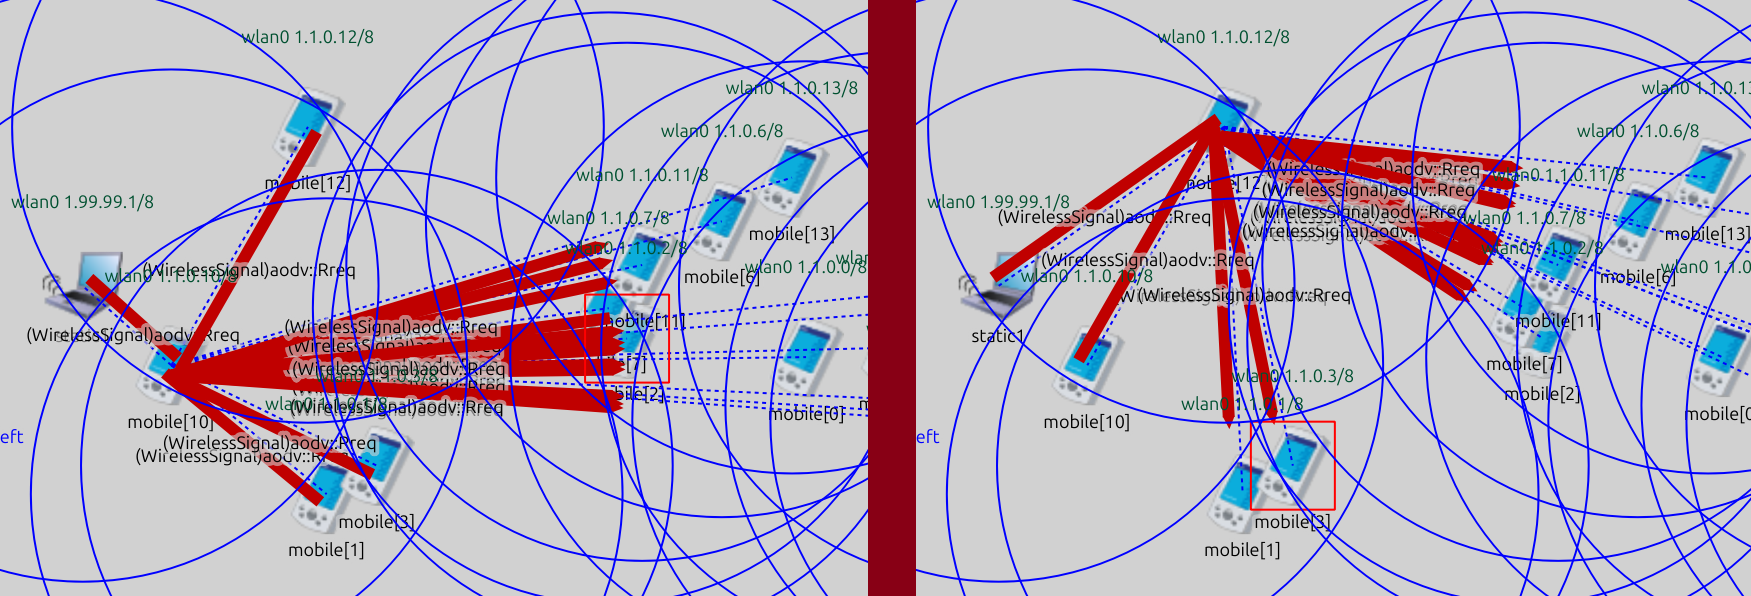
\includegraphics[width=135mm, scale=0.75]{imaxes/ejercicio1_2.png}
    \caption{Nodos que reenvían el primer RREQ (A la izquierda, mobile[10]; A la derecha, mobile[12])}
    \label{fig:primer_rreq_transmission}
\end{figure}


\section{Ejercicio 1.2}

\subsection{Elige el nodo intermedio de la ruta que sigue el primer paquete RREQ que llega a static2. Muestra su tabla
de enrutamiento (vector <Ipv4route *> dentro del módulo ipv4.routingTable) justo antes y justo después de
recibir el primer RREQ. Explica las diferencias y cómo se crean las entradas que aparecen (incluyendo los campos
más importantes).}

\section{Ejercicio 1.3}

\subsection{Haz lo mismo justo antes y justo después del primer RREP.}

\section{Ejercicio 1.4}

\subsection{Tras aplicar la nueva configuración, ¿Cuál es el primer nodo en darse cuenta de la caída? ¿Cómo? Muestra una captura del log del nodo que se da
cuenta que muestre el motivo. ¿Notifica este nodo la caída del nodo?}

\section{Ejercicio 1.5}

\subsection{Muestra el contenido del paquete RERR en Wireshark explicando los campos más importantes. ¿Qué IP
tiene como destino? ¿Por qué?}

\section{Ejercicio 1.6}

\subsection{Explica cómo se propaga el RERR por la red. ¿Qué nodos lo reenvían? ¿Cómo sabe un nodo si debe reenviar
el RERR?}

\section{Ejercicio 1.7} 

\subsection{Muestra capturas de la tabla de enrutamiento de un nodo antes y después de recibir un RERR y explica en
qué cambia.}

\section{Ejercicio 1.8}

\subsection{¿Qué hace static1 al recibir el RERR? Muestra el contenido del siguiente RREQ en Wireshark. ¿En qué cambia
con respecto al de la pregunta 1?}
 \chapter{DSDV}
\label{chap:dsdv}

\section{Ejercicio 2.1}

\subsection{Avanza la simulación hasta el instante t = 7 s. Busca el primer paquete Hello transmitido a partir a ese
instante con un valor de hopdistance de al menos 3 y muestra una captura del contenido. Explica el significado
de los campos srcAddress y nextAddress, utilizando para explicarlos una captura de la tabla de enrutamiento del
nodo que está transmitiendo el paquete (i.e., no el que consta en srcAddress)}

\begin{figure}[H]
    \centering
    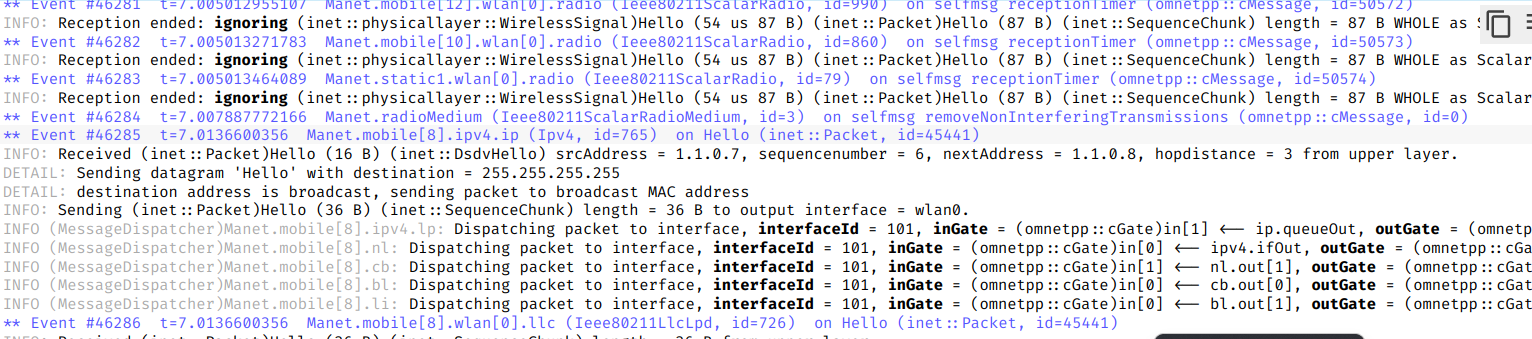
\includegraphics[width=155mm, scale=0.75]{imaxes/dsdv/ejercicio2_1.png}
    \caption{Log del nodo que manda el primer Hello con hopdistance 3}
    \label{fig:ejer2_1}
\end{figure}

Como se puede ver la imagen, el nodo que manda el primer mensaje Hello con hopdistance 1 es el nodo 8. Vamos a fijarnos en su tabla de enrutamiento:

\begin{figure}[H]
    \centering
    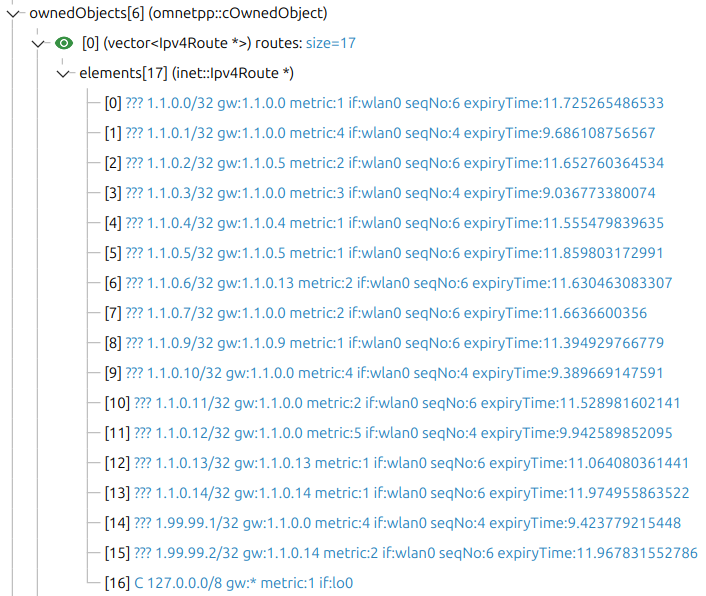
\includegraphics[width=115mm, scale=0.75]{imaxes/dsdv/ejercicio2_1_2.png}
    \caption{Tabla de enrutamiento nodo 8}
    \label{fig:ejer2_1}
\end{figure}

Según la imagen \ref{fig:ejer2_1}, el campo srcAddress es el nodo que envía el paquete Hello, en este caso es el 1.1.0.7 y el campo nextAddress es la siguiente dirección que va a recibir la trama, en este caso 1.1.0.8. 



\section{Ejercicio 2.2}

\subsection{¿Qué valor tiene de sequencenumber? ¿Qué quiere decir ese valor?}

\section{Ejercicio 2.3}

\subsection{¿Cómo se modifica? ¿Qué nodo lo modifica, y cuándo lo hace?}

\section{Ejercicio 2.4}

\subsection{Muestra la tabla de enrutamiento del nodo que recibe el Hello de la pregunta anterior justo antes y justo
después de recibirlo, relacionándola con el contenido del paquete. Si se actualiza la tabla, explica por qué se
actualiza y las entradas que se crean. Si no se actualiza, explica por qué no se actualiza y di qué entrada se
crearía (destino, gateway, métrica) si se actualizase con la información del paquete.}

\section{Ejercicio 2.5}

\subsection{Avanza hasta la caída del nodo en t = 15 s. Ten en cuenta que la ruta en ese momento puede ser diferente a
la de AODV, y por lo tanto el nodo a desactivar también. ¿Cuál es el primer nodo en darse cuenta de la caída?
¿Notifica la caída del nodo de alguna forma?}

\section{Ejercicio 2.6}

\subsection{¿Cómo se repara la ruta entre static1 y static2? ¿En qué momento?}

 
 \chapter{AODV vs. DSDV}
\label{chap:aodvdsdv}

\section{Ejercicio 3.1}

\subsection{¿En qué instante se realiza la primera transmisión (de cualquier tipo de paquete) con AODV? ¿Y con DSDV?
¿Por qué?}

La primera transmisión de AODV se hace a los 10.002 segundos. En cambio, DSDV transmite el primer paquete a los 0.056 segundos.

La diferencia que hay es debido a que DSDV es un protocolo proactivo, por lo que va actualizando cada poco tiempo las tablas de enrutamiento para así mantener la información fresca. En cambio AODV es un protocolo reactivo, solo manda paquetes cuando es necesario.

\section{Ejercicio 3.2}

\subsection{¿En qué instante recibe static2 el datagrama UdpBasicAppData-0 con AODV? ¿Y con DSDV? ¿Por qué?}

Con AODV static2 recibe el datagrama a los 11.4526 segundos, mientras que con DSDV lo recibe a los 10.0030 segundos. Esto ocurre porque en AODV los nodos tienen que ir actualizando la tabla de enrutamiento para poder encontrar la ruta y esto lleva un tiempo extra, en cambio en DSDV al tener todos los nodos sus tablas actualizadas, a la hora que querer establecer la ruta ya lo hace al instante.


\section{Ejercicio 3.3}

\subsection{¿Cuántos paquetes se pierden como consecuencia de la caída del nodo en AODV? ¿Y en DSDV? ¿A qué se
debe la diferencia? (Nota: para calcular el número de paquetes perdidos avanza hasta un instante posterior a la
caída en el que en ambos escenarios static2 vuelva a recibir datagramas y calcula la diferencia entre el número
de paquetes recibidos en static2 con y sin la caída del nodo).}

Para el caso de DSDV tuvimos que usar la semilla 65634 para poder ver con claridad la pérdida de paquetes y asi hacer la comparación.

Hemos hecho las simulaciones en ambos casos hasta los 22 segundos y en la tabla \ref{tabla1} se ven los resultados:

\begin{table}[H]
    \centering
    \begin{tabular}{|c|c|c|c|}
    \hline
    Protocolo & Sin fallo & Con fallo & \% pérdidas \\ \hline
      AODV    &   325     &   323     &     0.6\%   \\ \hline
      DSDV    &   254     &   156     &     38.5\%  \\ \hline
    \end{tabular}
    \caption{Tabla comparativa pérdida paquetes al caer un nodo}
    \label{tabla1}
\end{table}

Como vemos, en AODV la pérdida de paquetes es irrisoria con respecto a DSDV. Esto se debe a que en AODV, cuando un nodo detecta un fallo en la ruta, este envía un RERR a todos los nodos para informarlos del error por lo que se empieza a buscar inmediatamente otra ruta alternativa. En cambio en DSDV, cuando un nodo detecta una ruta inválida, no se genera otra ruta hasta que todos los nodos tengan su tabla de enrutamiento actualizada por lo que esto se traduce a una pérdida significativa de paquetes ya que tardan en actualizar sus tablas un cierto período de tiempo. 

\section{Ejercicio 3.4}

\subsection{Con la caída del nodo desactivada, simula AODV y DSDV durante 300 s (sim-time-limit). Muestra
capturas de los nodos estáticos a nivel de aplicación (doble click sobre el nodo) al final de la simulación. ¿Qué
porcentaje de los UdpBasicAppData enviados por static1 llega a static2? Explica los valores y las diferencias
observadas}

Primero vamos a ver lo que pasa en AODV, para eso vamos a fijarnos en las siguientes imágenes:

\begin{figure}[H]
    \centering
    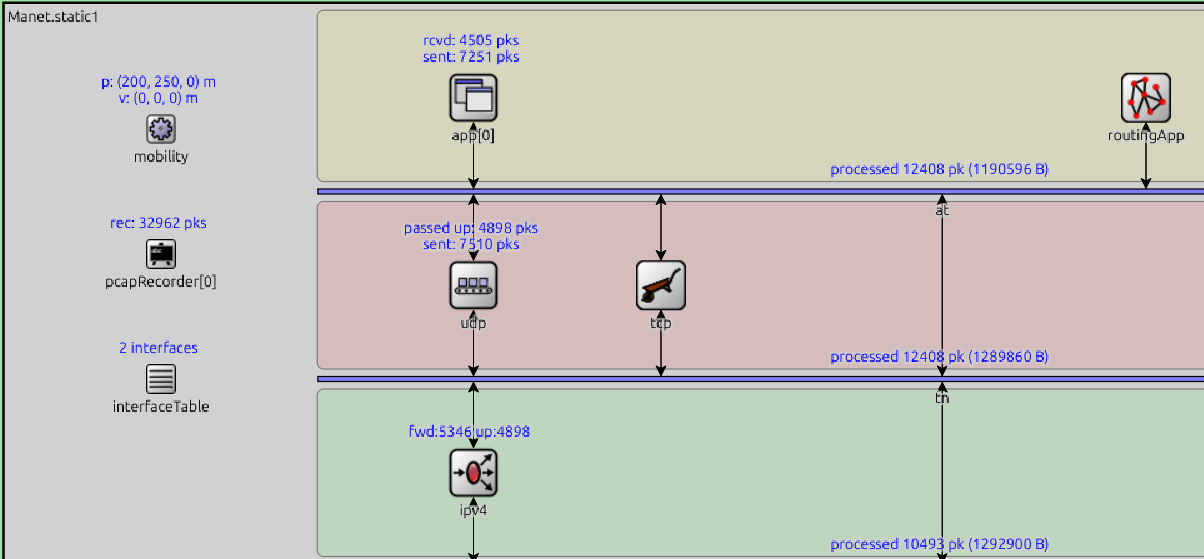
\includegraphics[width=155mm, scale=0.75]{imaxes/aodv_dsdv/ejercicio3_4_static1_aodv.png}
    \caption{Static1 a los 300s en AODV}
    \label{fig:ejer3_4_1}
\end{figure}

\begin{figure}[H]
    \centering
    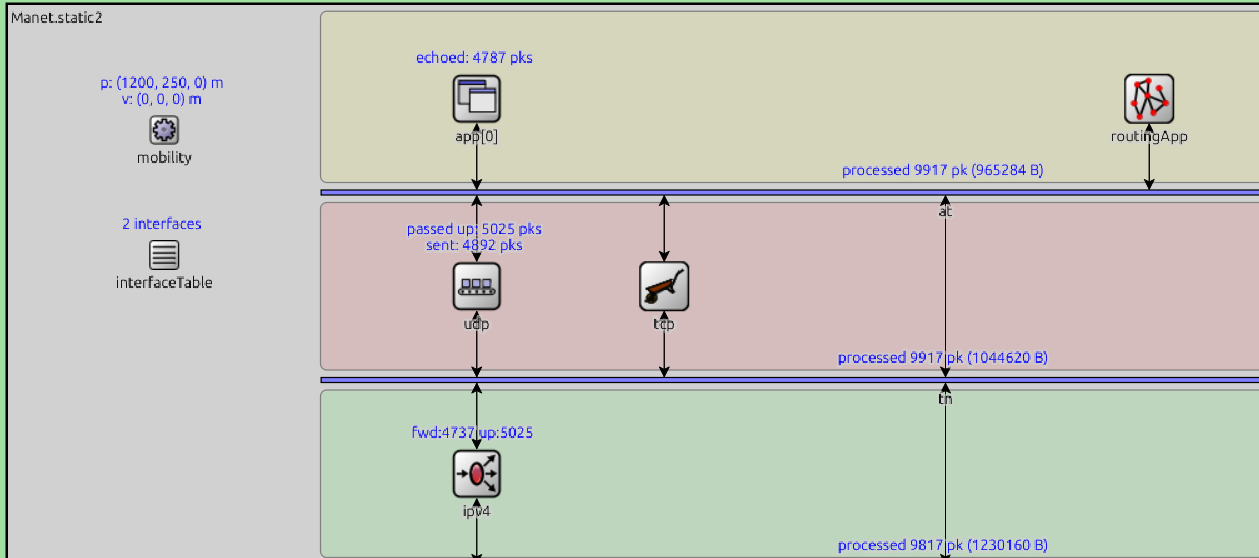
\includegraphics[width=155mm, scale=0.75]{imaxes/aodv_dsdv/ejercicio3_4_static2_aodv.png}
    \caption{Static2 a los 300s en AODV}
    \label{fig:ejer3_4_2}
\end{figure}

Como vemos, en la imagen \ref{fig:ejer3_4_1}, static1 manda 7251 paquetes y static2 recibe 4787 (imagen \ref{fig:ejer3_4_2}), por lo que se traduce a que a static2 le llega el 66\% de los paquetes.

Ahora vamos a ver lo que pasa en DSDV:

\begin{figure}[H]
    \centering
    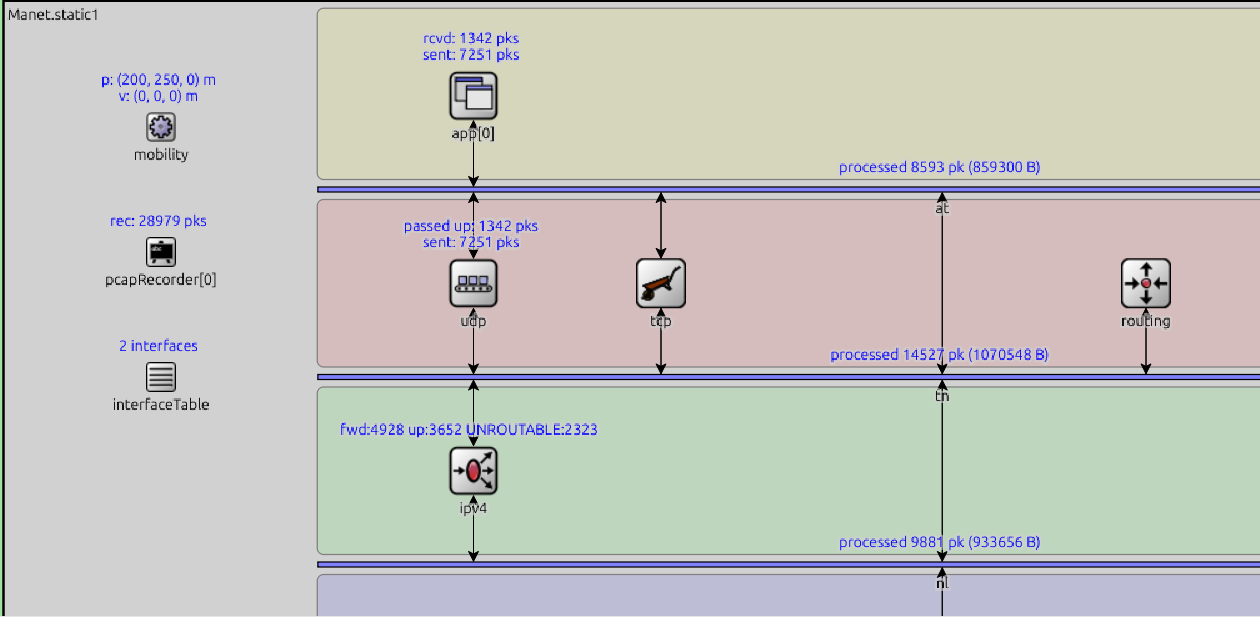
\includegraphics[width=155mm, scale=0.75]{imaxes/aodv_dsdv/ejercicio3_4_static1_dsdv.png}
    \caption{Static1 a los 300s en DSDV}
    \label{fig:ejer3_4_3}
\end{figure}

\begin{figure}[H]
    \centering
    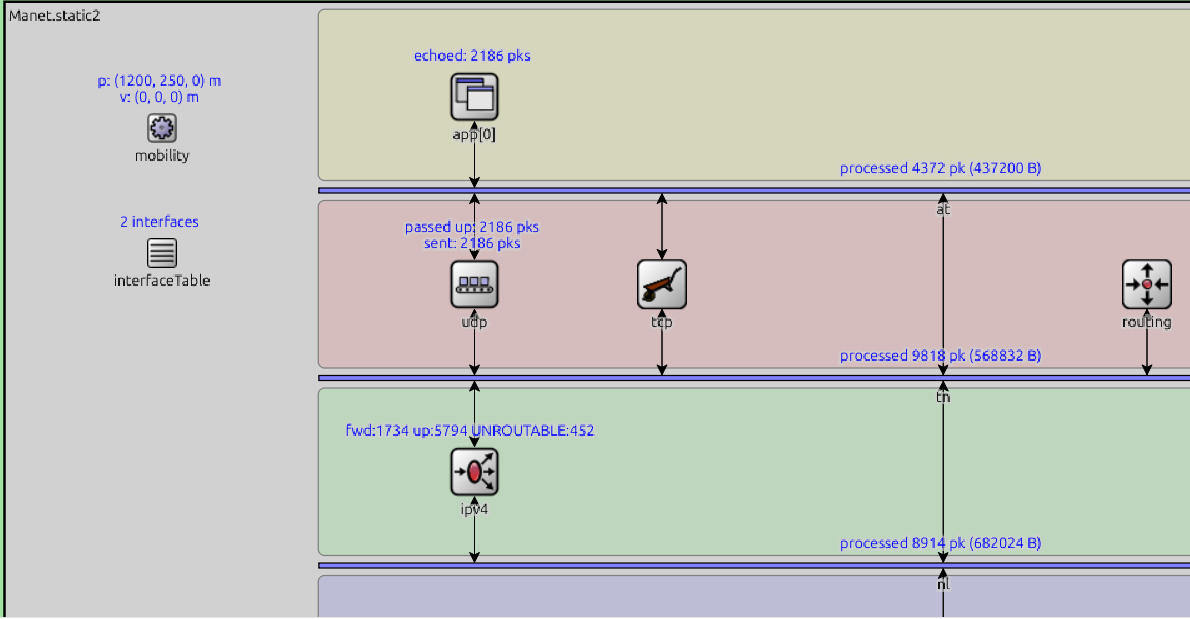
\includegraphics[width=155mm, scale=0.75]{imaxes/aodv_dsdv/ejercicio3_4_static2_dsdv.png}
    \caption{Static2 a los 300s en DSDV}
    \label{fig:ejer3_4_4}
\end{figure}

Si vemos la imagen \ref{fig:ejer3_4_3}, static1 manda 7251, mientras que a static2 le llegan 2186 (ver imagen \ref{fig:ejer3_4_4}), por lo que solamente le llega a static2 el 30\%.

La diferencia que hay entre AODV y DSDV es muy grande. Concretamente, DSDV pierde el doble de los paquetes con respeto AODV. Esto se debe a la constante actualización de las tablas de enrutamiento que hay en DSDV, por lo que cambia constantemente de ruta, mientras que en AODV cuando detecta una ruta, se mantiene todo el tiempo activa hasta que no sea válida. Además, en DSDV cuando se cambia de ruta o deja de ser válida, tiene que volver a hacer el proceso de reconstrucción y esto se traduce en un período de tiempo que static2 no recibe ningún paquete de static1. 


\section{Ejercicio 3.5}

\subsection{¿Qué porcentaje de los paquetes devueltos por static2 llegan a static1? Explica los valores y las diferencias
observadas.}

Para el caso de AODV, static2 hace echo de los 4787 paquetes que recibe y static1 recibe 4505 paquetes (imagen \ref{fig:ejer3_4_1}), por lo que esto lleva a que static1 recibe el 94\% de los paquetes que le manda static2.

En DSDV, static2 manda 2186 paquetes y static1 recibe 1342 paquetes (imagen \ref{fig:ejer3_4_3}), por lo que se traduce a que static1 recibe el 61\% de los paquetes mandados por static2. 

La diferencia que hay entre AODV y DSDV es dado a como funciona cada protocolo. AODV por cada RREQ que se manda entre los nodos, hay un RREP haciendo la ruta inversa por por la misma ruta que se ha establecido de ida, por lo que es más difícil de que haya pérdida de paquetes. En cambio, en DSDV al no haber un control en la ruta inversa, si algún nodo no es capaz de poder devolver el paquete, se pierde entonces hasta que tenga una ruta de vuelta actualizada/disponible. También hay que comentar que en DSDV hay una mayor congestión en el tráfico, por lo que se puede provocar colisiones y sobrecargas.
 \chapter{AODV vs. DSDV: gráficas}
\label{chap:aodv_dsdv_graf}


\section{Ejercicio 4.1}
\subsection{Obtén una gráfica que muestre el número de paquetes recibidos por static2 en función de la potencia tanto
para AODV como para DSDV}

\begin{figure}[H]
    \centering
    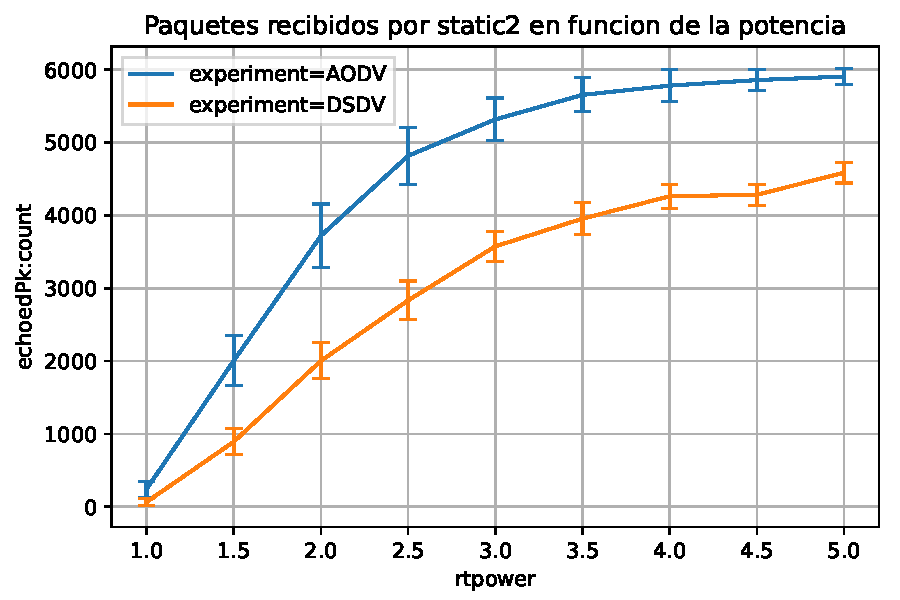
\includegraphics{imaxes/graficas/ejer4_1.pdf}
    \caption{Gráfica paquetes recibidos en static2 en función de la potencia}
    \label{fig:ejer4_1}
\end{figure}

\section{Ejercicio 4.2}

\subsection{Obtén una gráfica similar para el número de nodos. Explica lo observado.?}

\section{Ejercicio 4.3}

\subsection{Obtén una gráfica como las anteriores para la velocidad. Explica lo observado.}

\begin{figure}[H]
    \centering
    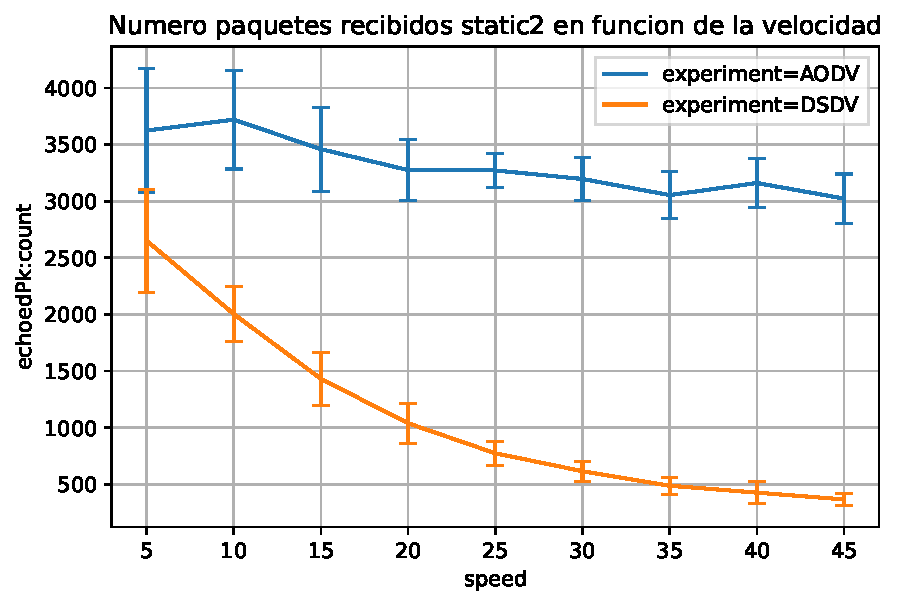
\includegraphics{imaxes/graficas/ejer4_3.pdf}
    \caption{Gráfica paquetes recibidos en static2 en función de la velocidad}
    \label{fig:ejer4_1}
\end{figure}

\section{Ejercicio 4.4}

\subsection{Para DSDV, obtén una gráfica del porcentaje de paquetes perdidos con diferentes valores de helloInterval.
Explica lo observado.}
 %\chapter{Otras Gráficas}
\label{chap:sinqos}

\begin{figure}[!ht]
    \centering
    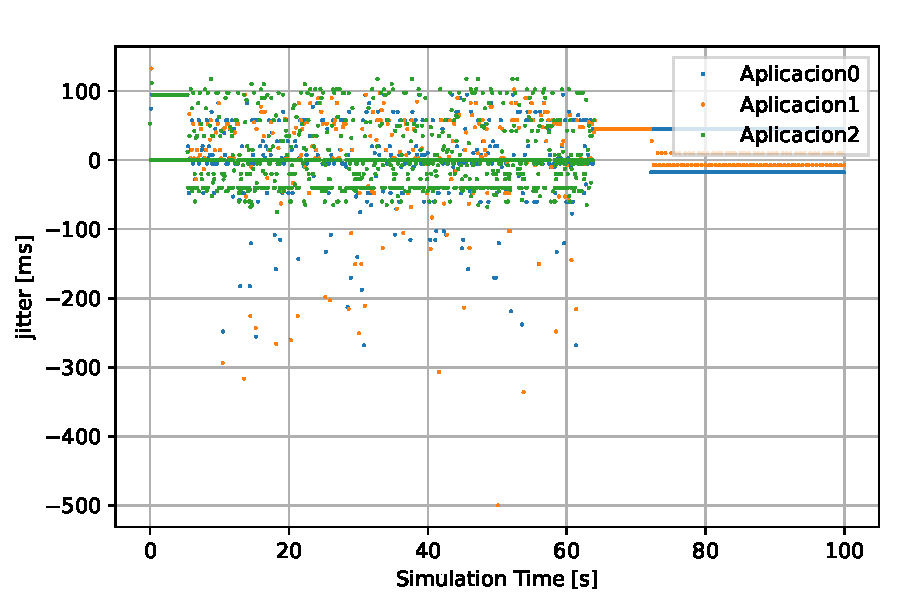
\includegraphics{graficas/sinQoS/jitter_SinQoS.pdf}
    \caption{Jitter a partir retardo extremo a extremo del router sin QoS}
    \label{fig:sinqos_jitter}
\end{figure}

\begin{figure}
    \centering
    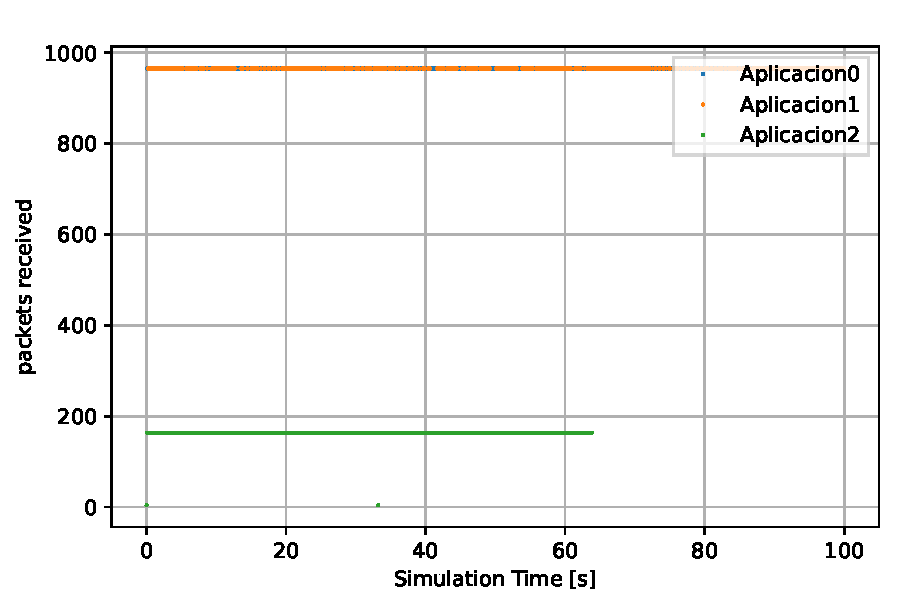
\includegraphics{graficas/sinQoS/packetsReceived_sinQoS.pdf}
    \caption{Paquetes recibidos en el servidor sin QoS}
    \label{fig:sinqos_pktreceived}
\end{figure}

\begin{figure}
    \centering
    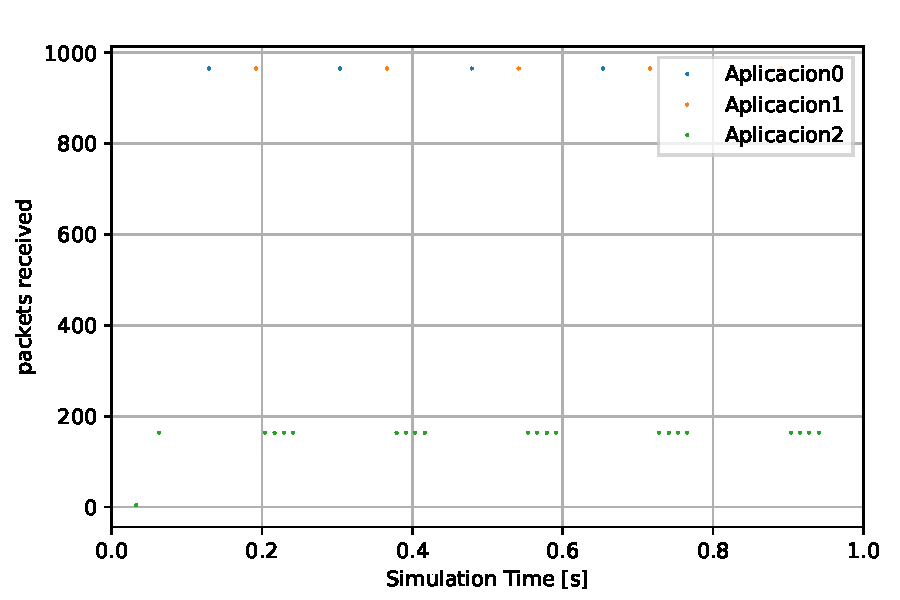
\includegraphics{graficas/sinQoS/packetsReceived_sinQoS_1.pdf}
    \caption{Paquetes recibidos en el servidor sin QoS intervalo 0-1}
    \label{fig:sinqos_pktreceived01}
\end{figure}

\begin{figure}
    \centering
    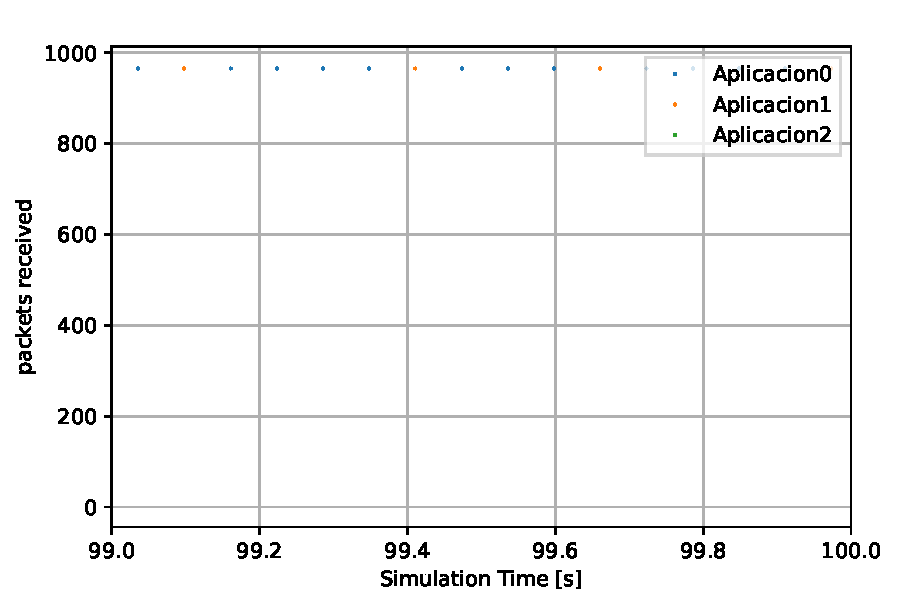
\includegraphics{graficas/sinQoS/packetsReceived_sinQoS_99.pdf}
    \caption{Paquetes recibidos en el servidor sin QoS intervalo 99-100}
    \label{fig:sinqos_pktreceived99100}
\end{figure}


\begin{figure}[!ht]
    \centering
    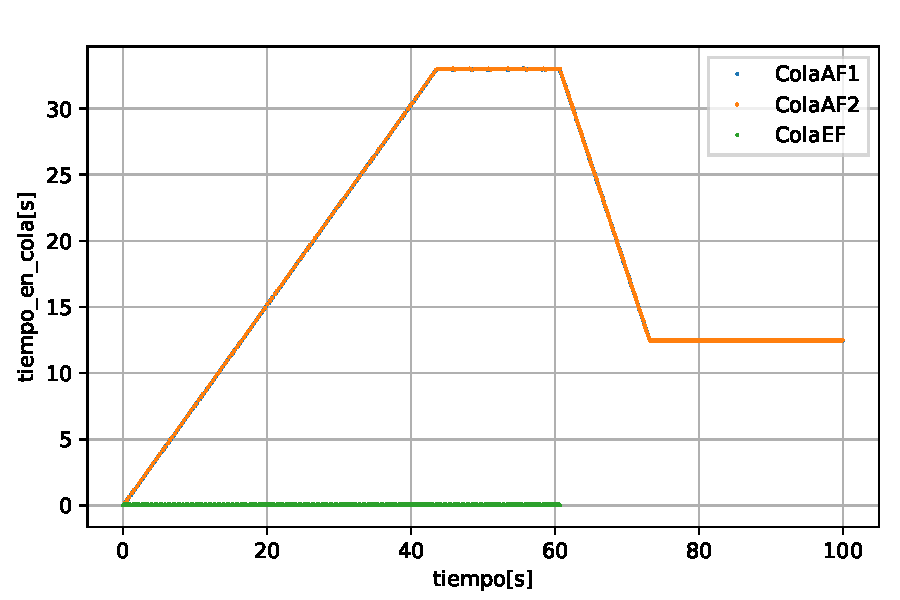
\includegraphics{graficas/DropTail/tiempo_en_cola_droptail.pdf}
    \caption{Tiempo encolado droptail}
    \label{fig:droptail_time}
\end{figure}

\begin{figure}
    \centering
    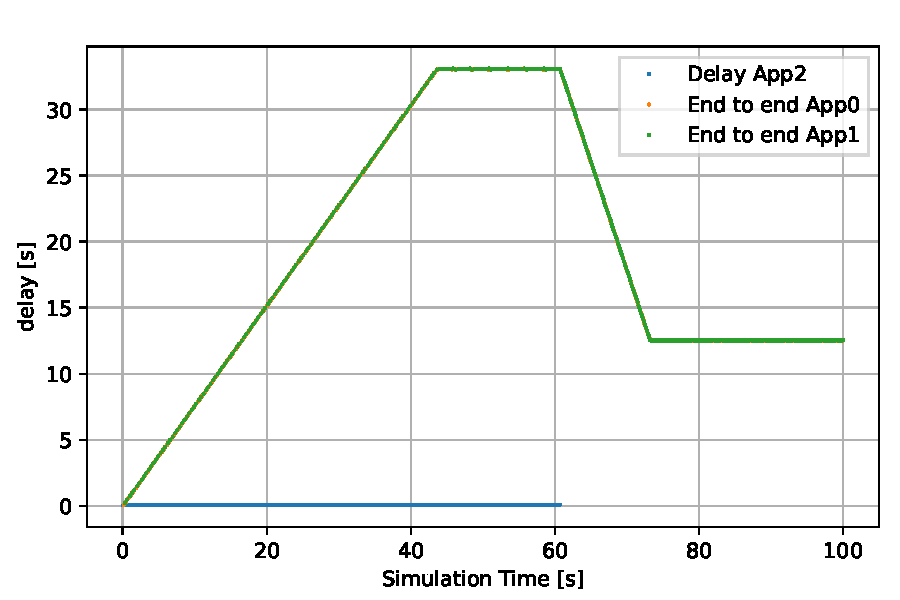
\includegraphics{graficas/DropTail/delay_DT.pdf}
    \caption{Delay extremo a extremo con droptail}
    \label{fig:sinqos_pktreceived99100}
\end{figure}

\begin{figure}
    \centering
    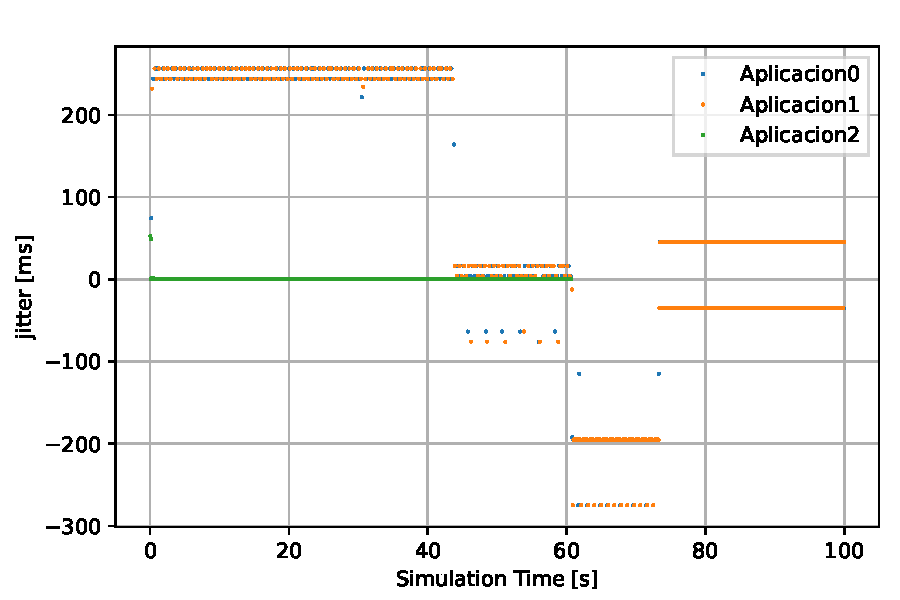
\includegraphics{graficas/DropTail/jitter_DT.pdf}
    \caption{Jitter a partir retardo extremo a extremo droptail}
    \label{fig:sinqos_pktreceived99100}
\end{figure}

\begin{figure}
    \centering
    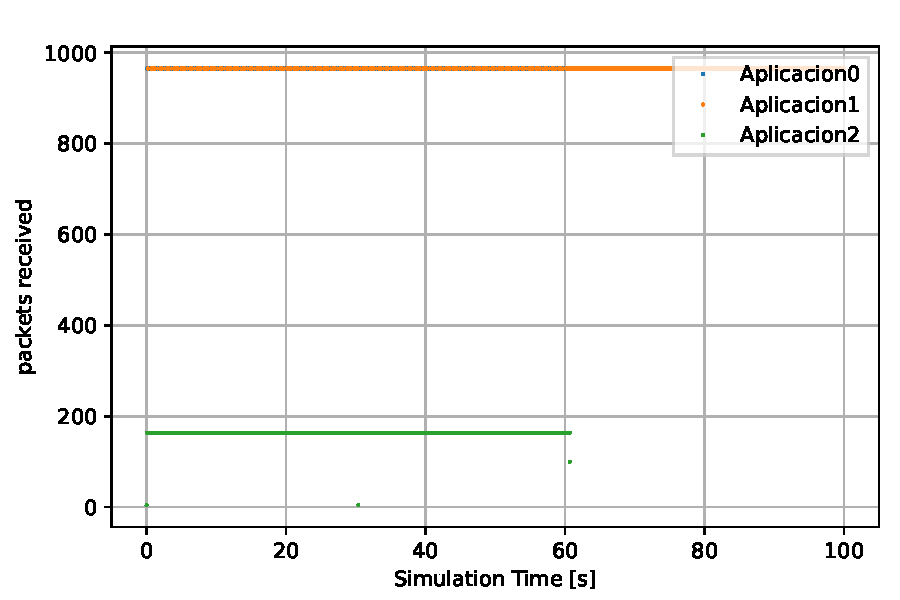
\includegraphics{graficas/DropTail/packetsReceived_DT.pdf}
    \caption{Paquetes recibidos en el servidor droptail}
    \label{fig:sinqos_pktreceived99100}
\end{figure}

\begin{figure}
    \centering
    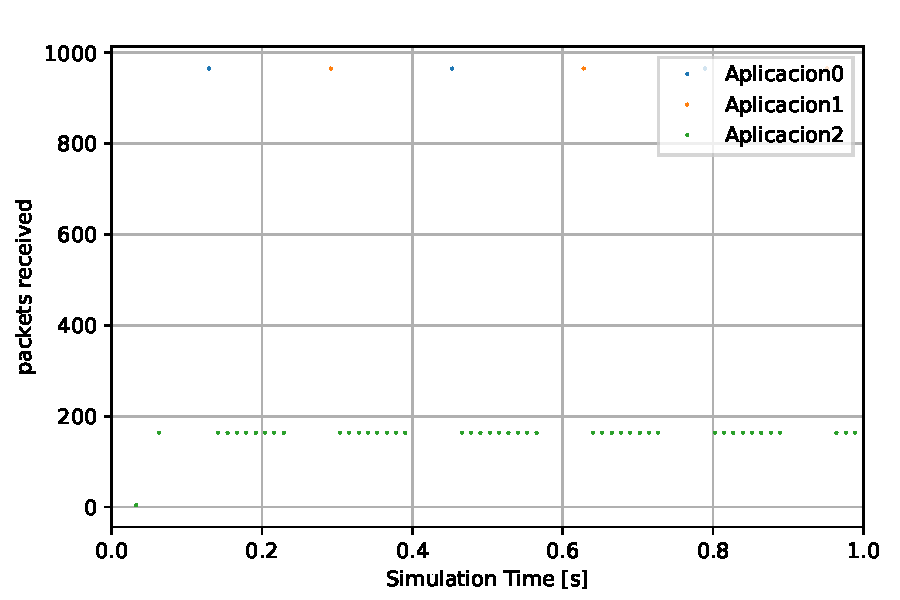
\includegraphics{graficas/DropTail/packetsReceived_DT_1.pdf}
    \caption{Paquetes recibidos en el sevidor droptail intervalo 0-1 }
    \label{fig:sinqos_pktreceived99100}
\end{figure}

\begin{figure}
    \centering
    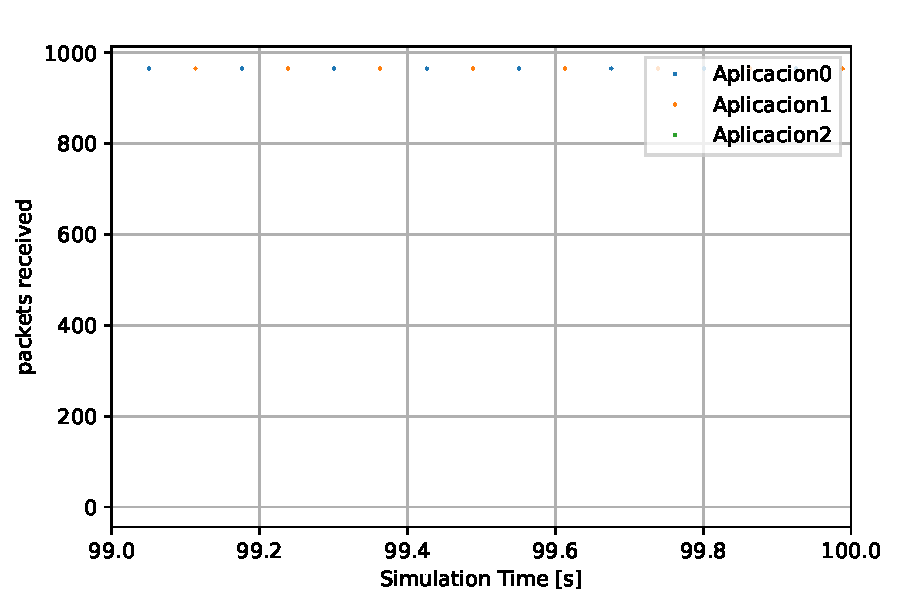
\includegraphics{graficas/DropTail/packetsReceived_DT_99.pdf}
    \caption{Paquetes recibidos en el servidor droptail intervalo 99-100}
    \label{fig:sinqos_pktreceived99100}
\end{figure}


\begin{figure}[!ht]
    \centering
    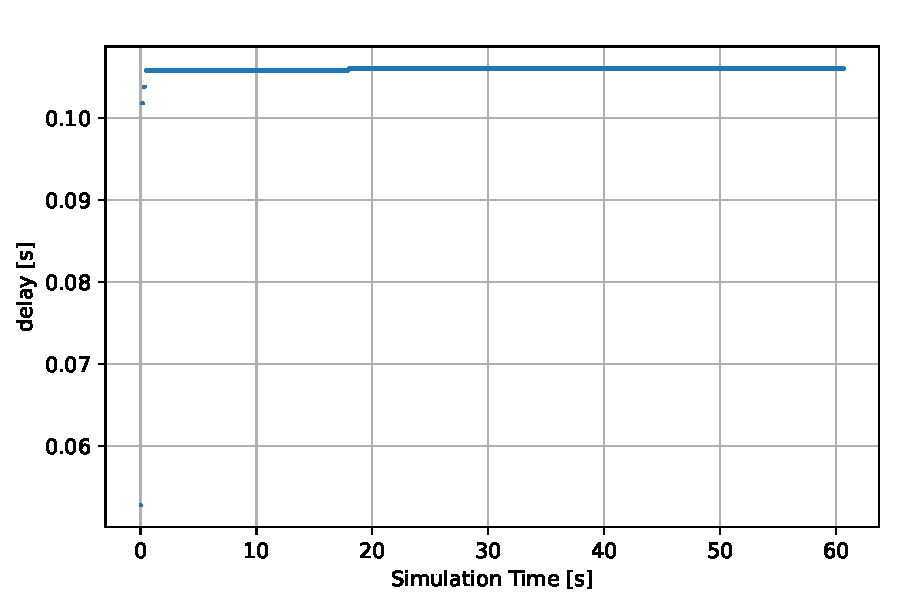
\includegraphics{graficas/WRR/delay_wrr.pdf}
    \caption{Retardo extremo a extremo WRR16}
    \label{fig:sinqos_pktreceived99100}
\end{figure}

\begin{figure}
    \centering
    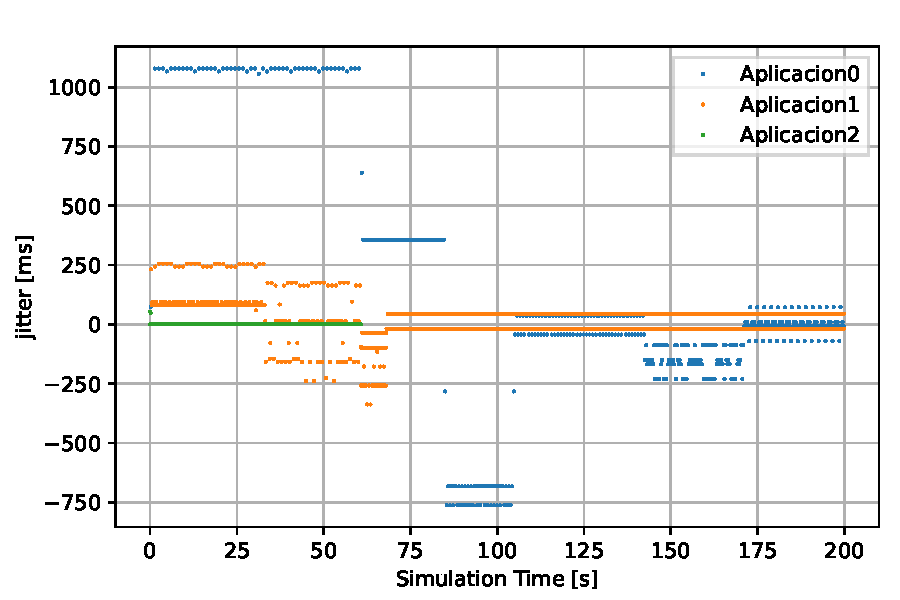
\includegraphics{graficas/WRR/jitter_WRR.pdf}
    \caption{Jitter a partir retardo extremo a extremo WRR16}
    \label{fig:sinqos_pktreceived99100}
\end{figure}

\begin{figure}
    \centering
    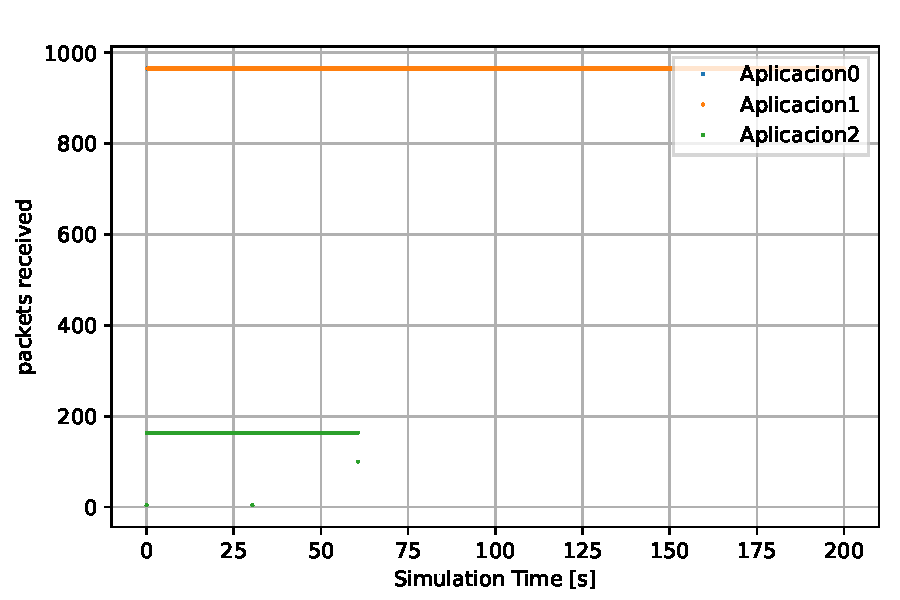
\includegraphics{graficas/WRR/packetsReceived_WRR.pdf}
    \caption{Paquetes recibidos en el servidor con WRR16}
    \label{fig:sinqos_pktreceived99100}
\end{figure}

\begin{figure}
    \centering
    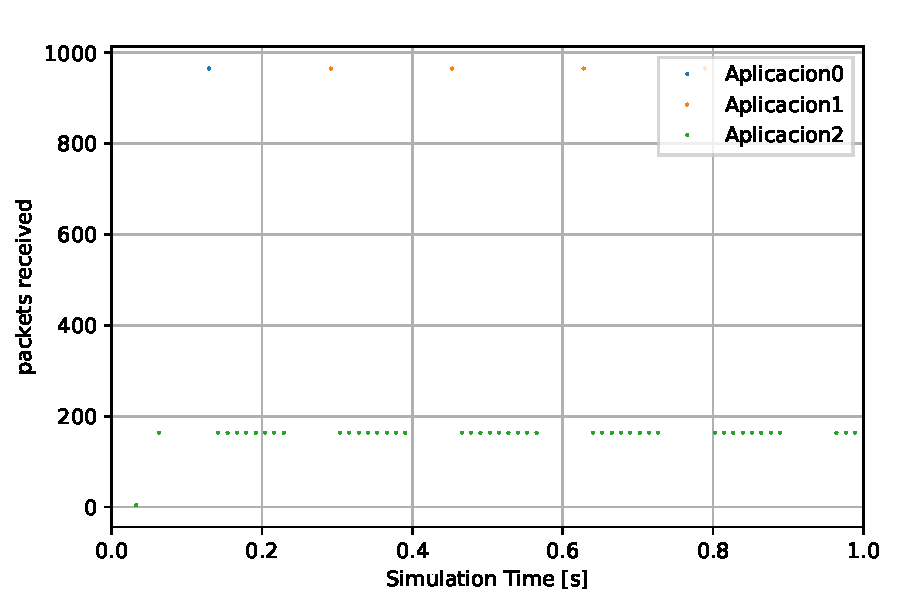
\includegraphics{graficas/WRR/packetsReceived_WRR_1.pdf}
    \caption{Paquetes recibidos en el servidor con WRR16 intervalo 0-1}
    \label{fig:sinqos_pktreceived99100}
\end{figure}

\begin{figure}
    \centering
    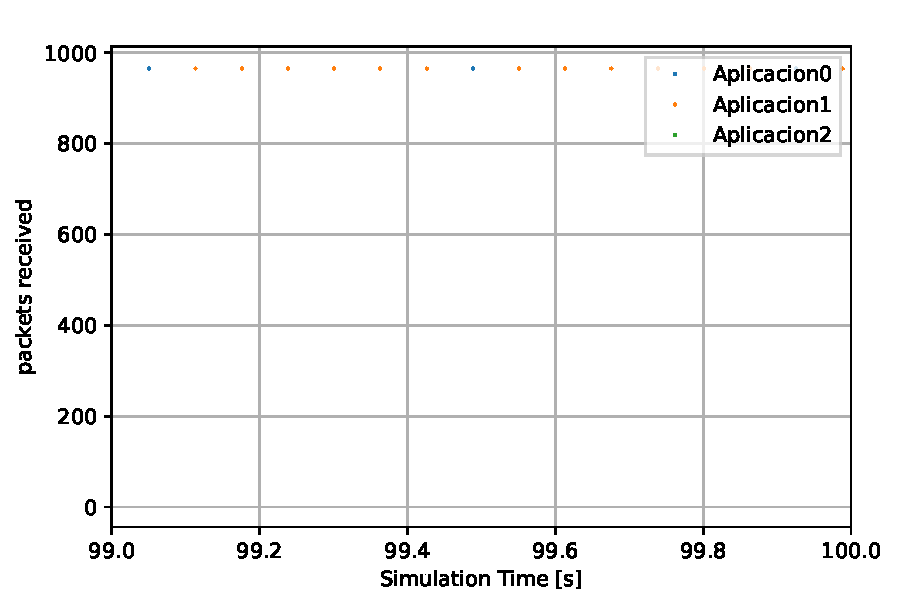
\includegraphics{graficas/WRR/packetsReceived_WRR_99.pdf}
    \caption{Paquetes recibidos en el servidor con WRR16 intervalo 99-100}
    \label{fig:sinqos_pktreceived99100}
\end{figure}

\begin{figure}
    \centering
    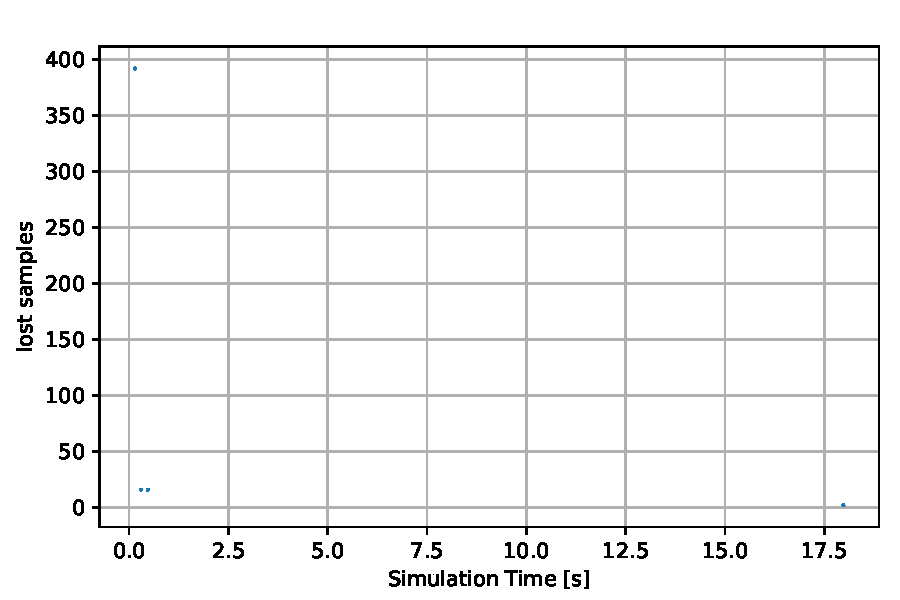
\includegraphics{graficas/WRR/muestras_perdidas_wrr.pdf}
    \caption{Muestras perdidas WRR16}
    \label{fig:sinqos_pktreceived99100}
\end{figure}


\begin{figure}[!ht]
    \centering
    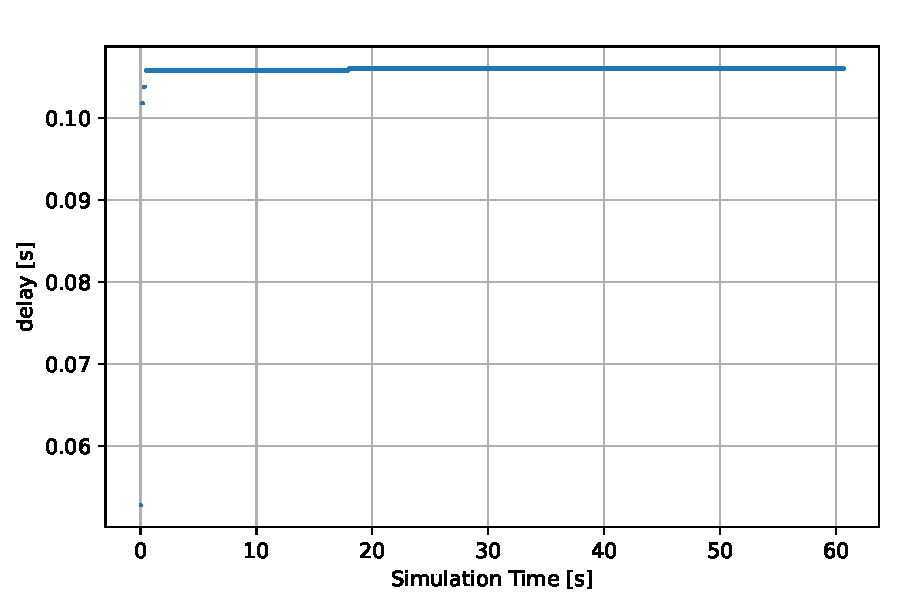
\includegraphics{graficas/RED/delay_red.pdf}
    \caption{Retardo extremo a extremo RED}
    \label{fig:sinqos_pktreceived99100}
\end{figure}

\begin{figure}
    \centering
    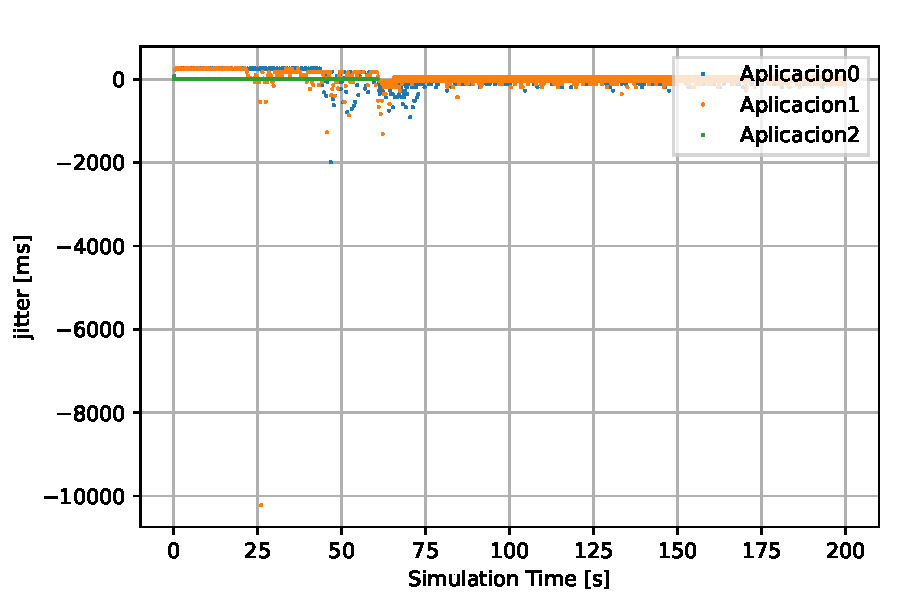
\includegraphics{graficas/RED/jitter_RED.pdf}
    \caption{Jitter a partir retardo extremo a extremo RED}
    \label{fig:sinqos_pktreceived99100}
\end{figure}

\begin{figure}
    \centering
    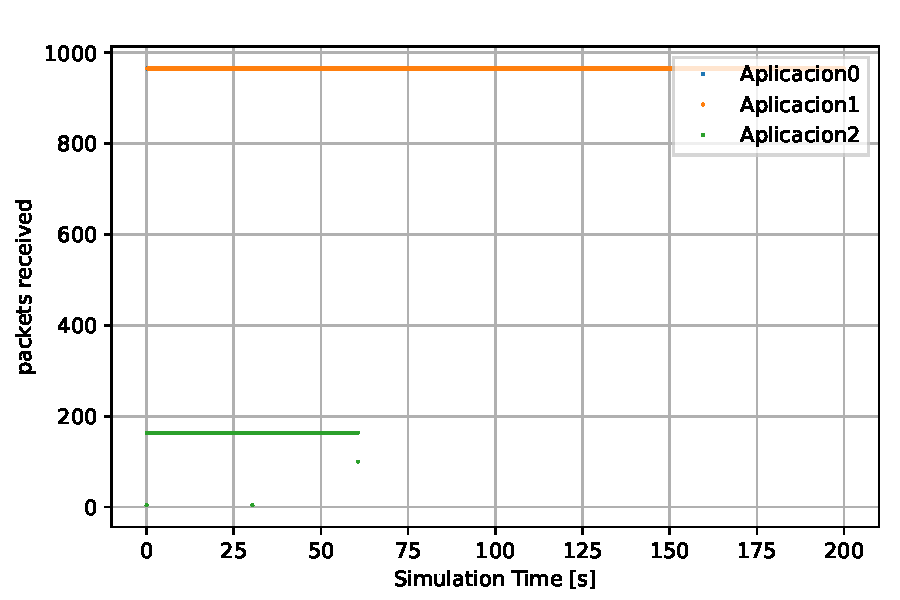
\includegraphics{graficas/RED/packetsReceived_RED.pdf}
    \caption{Paquetes recibidos en el servidor con RED}
    \label{fig:sinqos_pktreceived99100}
\end{figure}

\begin{figure}
    \centering
    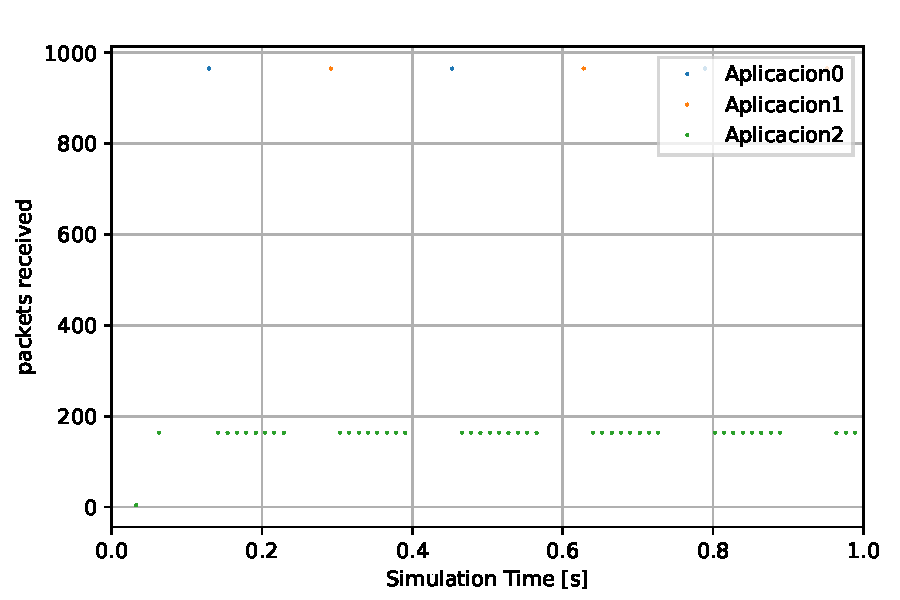
\includegraphics{graficas/RED/packetsReceived_RED_1.pdf}
    \caption{Paquetes recibidos en el servidor con RED intervalo 0-1}
    \label{fig:sinqos_pktreceived99100}
\end{figure}

\begin{figure}
    \centering
    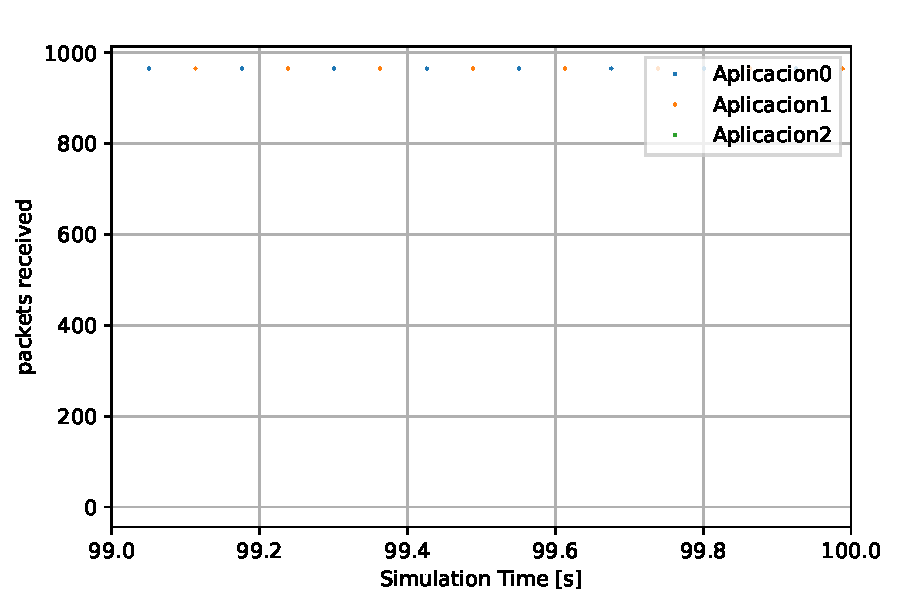
\includegraphics{graficas/RED/packetsReceived_RED_99.pdf}
    \caption{Paquetes recibidos en el servidor con RED intervalo 99-100}
    \label{fig:sinqos_pktreceived99100}
\end{figure}

\begin{figure}
    \centering
    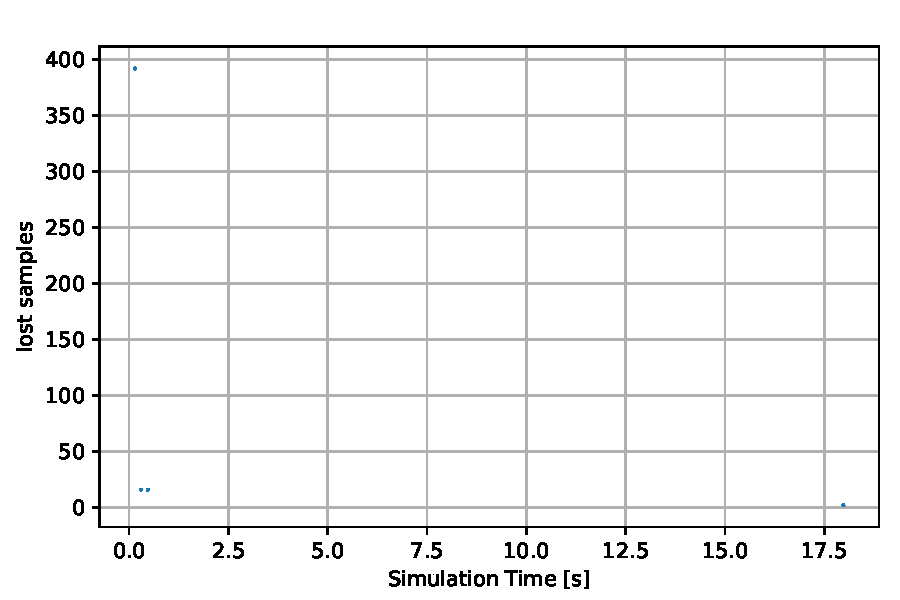
\includegraphics{graficas/RED/muestras_perdidas_red.pdf}
    \caption{Muestras perdidas con RED}
    \label{fig:sinqos_pktreceived99100}
\end{figure}




 %%%%%%%%%%%%%%%%%%%%%%%%%%%%%%%%%%%%%%%%
 % Apéndices, glosarios e bibliografía  %
 %%%%%%%%%%%%%%%%%%%%%%%%%%%%%%%%%%%%%%%%

%\appendix
%\appendixpage
%\chapter{Material adicional}
\label{chap:adicional}

\lettrine{E}{xemplo} de capítulo con formato de apéndice, onde se pode
incluír material adicional que non teña cabida no corpo principal do
documento, suxeito á limitación de 80 páxinas establecida no
regulamento de TFGs.

\Blindtext

%\include{anexos/...}

%\printglossary[type=\acronymtype,title=\nomeglosarioacronimos]
%\printglossary[title=\nomeglosariotermos]

%\bibliographystyle{IEEEtranN}
%\bibliography{\bibconfig,bibliografia/bibliografia}
%\clearpage
 
\end{document}

%%%%%%%%%%%%%%%%%%%%%%%%%%%%%%%%%%%%%%%%%%%%%%%%%%%%%%%%%%%%%%%%%%%%%%%%%%%%%%%%
